% !TEX root = main.tex

\section{操作系统概述}
\subsection{概述}
操作系统核心即怎么虚拟多几个冯诺依曼计算机出来给程序用。
操作系统是控制应用程序执行的程序,是应用程序和计算机硬件间的接口(屏蔽硬件细节)。

这里先解释几个概念
\begin{itemize}
	\item 并发:两件事情\textbf{可以}同时(simultaneously)发生,没有时间限制,$t_1>t_2$,$t_1<t_2$,$t_1=t_2$都可
	\item 同步:两个事件有确定的时间限制
	\item 异步:两件事不知道何时发生
\end{itemize}

并发和共享是操作系统两个最基本的特征

% 对称多处理器(symmetric multiple processors, SMP):共享内存(访存时间大致相同)、IO设备,所有处理器/核可执行相同功能(对称性)

\subsection{发展历史}
\begin{itemize}
	\item 串行处理/手工操作(1940s):没有OS,人工调度,准备时间长
	\item 简单批处理系统(1950s):
	\begin{itemize}
		\item 使用监控程序(monitor),读入用户程序执行
		\item 提供内存保护、计时器、特权指令、中断
		\item 两种操作模式:用户态、内核态(mode)
		\item 单道程序(uniprogramming)批处理:处理器必须等到IO指令结束后才能继续
	\end{itemize}
	\item 多道程序批处理(1950s末):多个作业同时进入主存,切换运行,\textbf{充分利用处理器}(大块处理时间,少交换上下文的调度);用户响应时间长,不提供人机交互能力
	\item 分时系统(1961):MIT CTSS(Compatible Time-Sharing System),满足用户与计算机交互的需要,\textbf{减小响应时间}(分时间片小块调度);多个交互作业,多个用户,把运行时间分成很短的时间片轮流分配
	\item 实时系统:专用,工业、金融、军事
\end{itemize}

现代的操作系统通常同时具有分时、实时核多道批处理的功能,因此被称为通用操作系统。
而OS也不仅是在PC机上有,网络OS、分布式OS、嵌入式OS层出不穷。

% OS发展中5个重要理论进展:进程、信息保护和安全、内存管理、调度和资源管理

影响现代OS发展的因素:
\begin{itemize}
	\item 新硬件:多核/处理器结构、高速增长的计算机速度、高速网络连接、容量的不断增加各种存储设备
	\item 新应用:多媒体应用、互联网/Web访问、客户/服务器计算模式
	\item 新安全威胁:网络使安全问题更突出(病毒、蠕虫、黑客技术)
\end{itemize}

% OS的组织方法和设计要素(现代OS的特征):微内核体系结构、多线程、对称多处理、分布式、面向对象设计

内核的分类:
\begin{itemize}
	\item 单体内核(monolithic kernel)/宏内核(macro kernel)
	\begin{itemize}
		\item 内核实现操作系统所有基本功能(包括调度、文件系统、连网、设备驱动程序、内存管理等等)
		\item 一般用一个进程实现,内核代码共享同一个地址空间,每一模块可以调用任意其它模块和使用内核所有核心数据
		\item 效率高,但难于修改和扩充
		\item 例子:Unix、Linux、Android(基于Linux)、DOS、Windows 9x、Mac OS 8.6以下
	\end{itemize}
	\item 微内核(microkernel)
	\begin{itemize}
		\item 内核只实现最基本功能(包括地址空间、IPC[InterProcess Communication,进程间通信]和基本调度)
		\item 更多的功能代码组织为多个进程,各自独立使用自己的地址空间,运行于用户态
		\item 一致接口(消息传递\footnote{即使是硬件中断也会被当作消息处理,需要send/receive})、可扩展性(允许增加新服务)、可移植性(将系统移植到新处理器只需对内核修改),适用于嵌入式与分布式环境,但效率稍低
		\item 例子:Mach、QNX
	\end{itemize}
	\item 混合内核
	\begin{itemize}
		\item 微内核与宏内核的结合(也可算作单体内核中的一类)
		\item 具有微内核结构,按宏内核实现
		\item 例子:Windows NT(2000/XP/Vista/7/8)、BSD、XNU(Darwin 的核心,源自Mach和BSD,用于Mac OS X 和iOS)
	\end{itemize}
\end{itemize}
\begin{figure}[H]
	\centering
	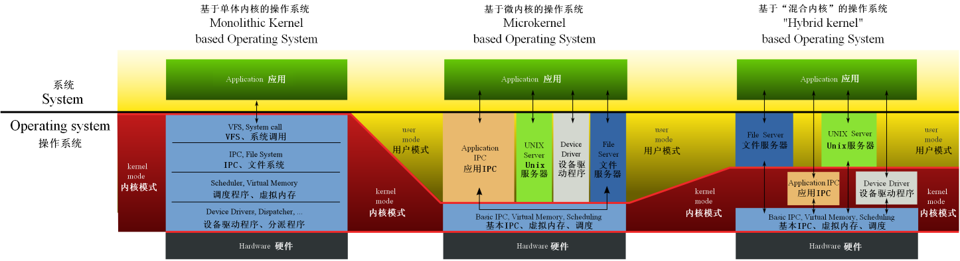
\includegraphics[width=\linewidth]{fig/kernels.png}
\end{figure}